\documentclass[xcolor=dvipsnames,split]{beamer}
% bibstuffs:
\usepackage[sort&compress]{natbib}
\bibliographystyle{apsr}
\bibpunct[:]{(}{)}{;}{a}{,}{,}

%\usepackage[all]{xy}
%\input xy
%\xyoption {all}




\usepackage{beamerthemesplit}
%\usecolortheme[rgb={0,0,.611764706}]{structure}
\definecolor{DukeBlue}{rgb}{0,0,.611764706}
\setbeamertemplate{items}[ball]
%\usetheme[height=11mm]{Rochester}
\usetheme[]{Boadilla} 

\definecolor{WUSTLgreen} {RGB} {44, 80, 54}
\definecolor{WUSTLred} {RGB} {149, 1, 1}
\definecolor{WUSTLtan} {RGB} {229, 210, 184}
\setbeamercolor{structure}{fg=WUSTLred, bg=WUSTLgreen}
\setbeamercolor{normaltext}{bg=black, fg=WUSTLtan}
\setbeamercolor{block title}{fg=WUSTLred}
\setbeamercolor{block title example}{fg=WUSTLgreen}
\setbeamercolor{frametitle}{fg=DukeBlue}
\setbeamercolor{title}{fg=DukeBlue}



\setbeamertemplate{blocks}[rounded]


\usepackage{rotating,amssymb,subfigure,tabularx}
\usepackage{caption}
\usepackage{graphicx}
\usepackage{color}
\usepackage{multicol}
\usepackage{array}
\usepackage{dcolumn}
\usepackage{multirow}
\usepackage{booktabs}
\usepackage{caption}
\setbeamerfont{tablefont}{size=\tiny}
\setbeamerfont{quotefont}{size=\small}


\newcommand{\bframe}{\begin{frame}}
\newcommand{\jacob}{\end{frame}}
\newcommand{\bi}{\begin{itemize}}
\newcommand{\ei}{\end{itemize}}
\newcommand{\be}{\begin{enumerate}}
\newcommand{\ee}{\end{enumerate}}
\newcommand{\vp}{\vspace{.5cm}}
\newcommand{\bis}{\begin{itemize}[<+->]}
\newcommand{\bes}{\begin{enumerate}[<+->]}
\newcommand{\red}[1]{\color{WUSTLred}{#1}}
\newcommand{\bc}{\begin{center}}
\newcommand{\ec}{\end{center}}
\newcommand{\eb}{\end{block}}
\newcommand{\ds}{\displaystyle}



\author[J. Montgomery, F. Hollenbach, M. Ward~~~~] 
{Jacob M. Montgomery  \inst{1} \and Florian M. Hollenbach  \inst{2} \and Michael D. Ward \inst{2}}


\institute[] % (optional, but mostly needed)
{
  \inst{1}%
Department of Political Science\\
Washington University in St. Louis
  \and
  \inst{2}%
  Department of Political Science\\
  Duke University}

 
\title[Election Night!]{\textsc{Say Yes to the Guess: \\ Combining Forecasts for the 2012 U.S. Presidential Election}}


\date{Nov. 6, 2012}


\begin{document}


\frame{\titlepage}


\section{Introduction}


\frame{


\bc
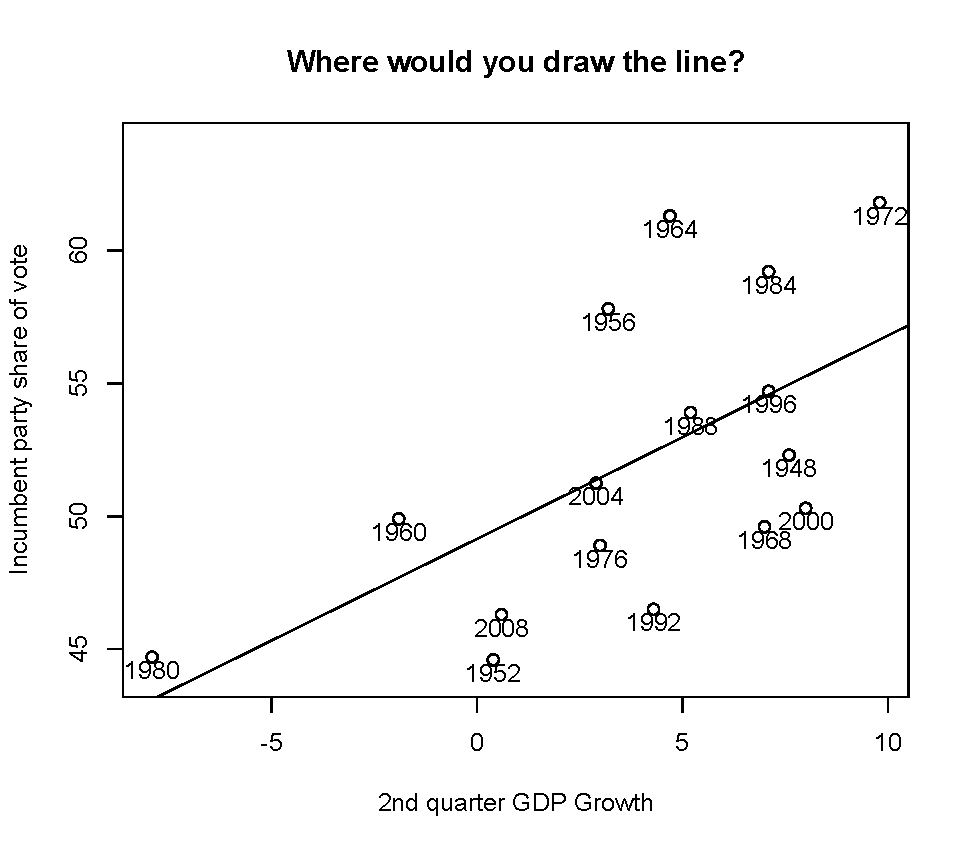
\includegraphics[width=4in]{GDPElections3}
\ec

}



\frame{


\bc
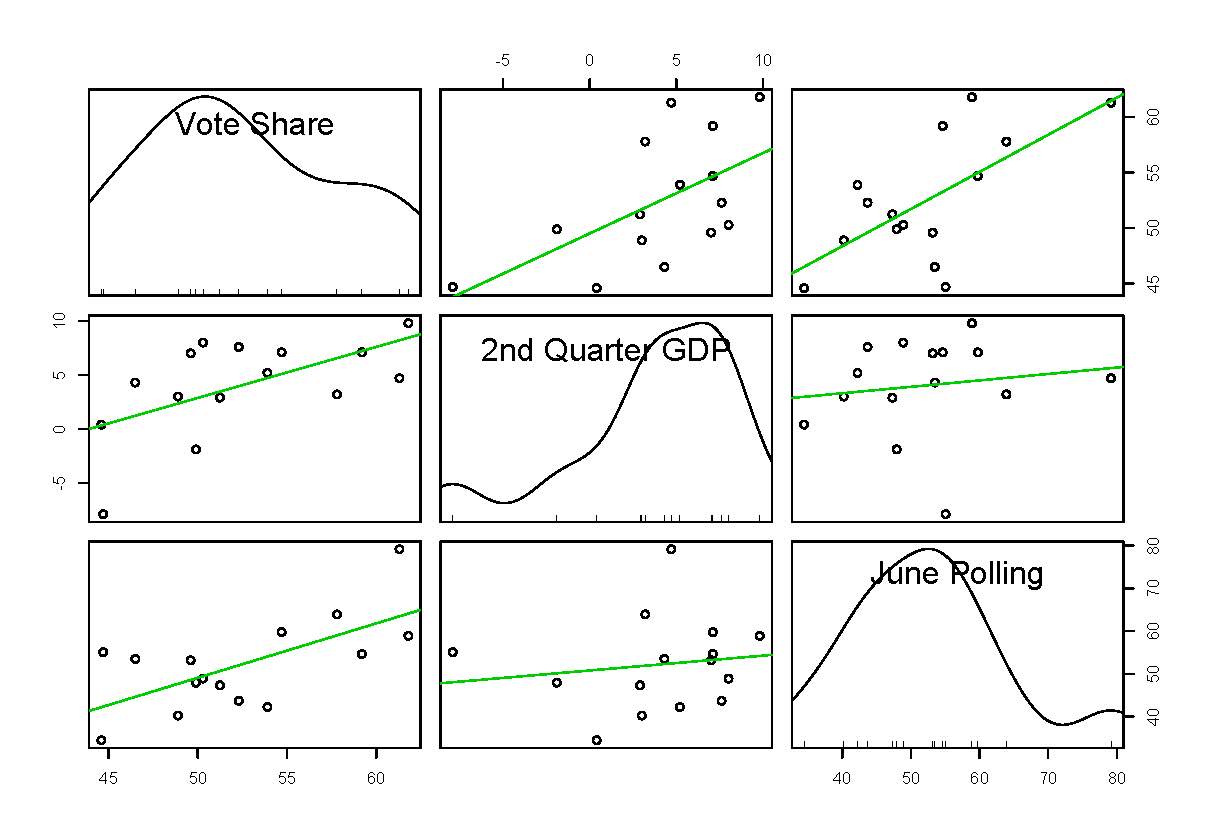
\includegraphics[width=5in]{ScatterPlotMatrix}
\ec

}


\frame{
\frametitle{Which can also be thought of like this}



\bc
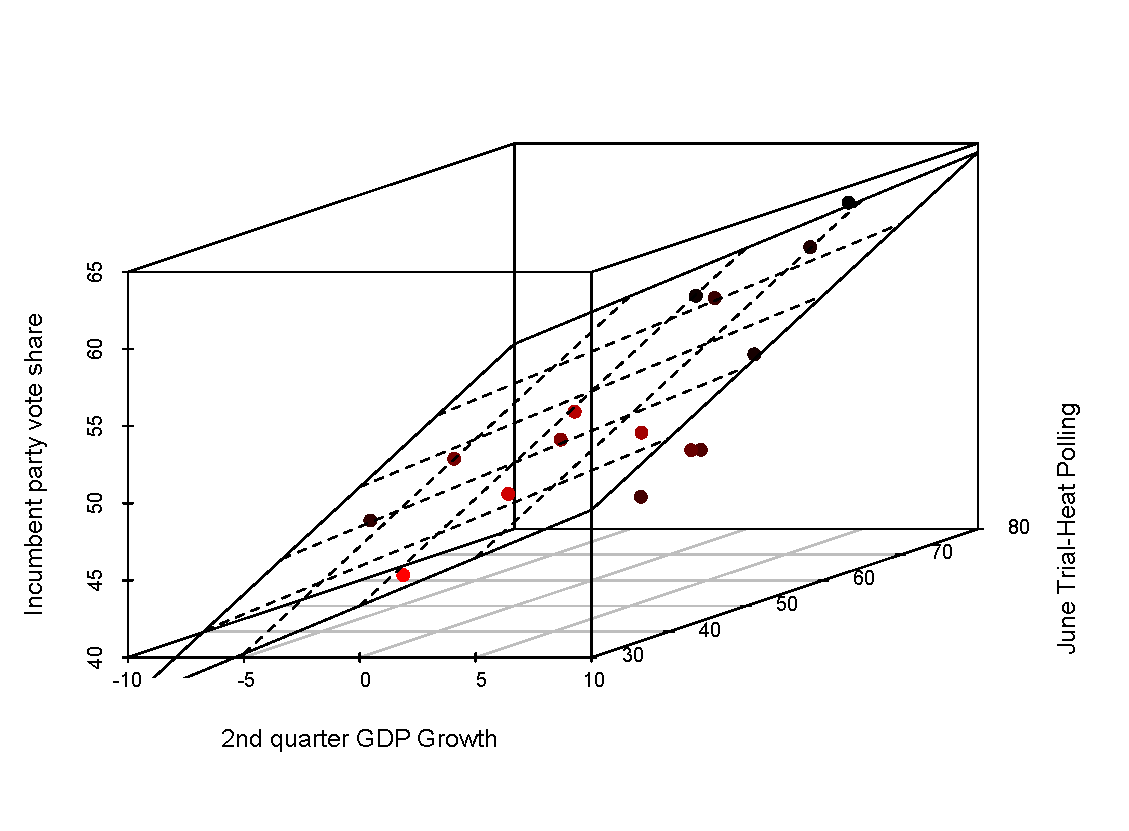
\includegraphics[width=4.4in]{ElectionsIn3D}
\ec

}







\frame{\frametitle{Predicting the Incumbent Voteshare in the 2012 Presidential Election}     

\begin{center}
\begin{footnotesize}
\begin{tabular}{rlrrrrrrrrr}
\toprule
  & F & A & C & H & LBRT & L & Hol & EW & Cuz \\ 
\midrule
  1992 & 55.7 & 46.3 & 49.7 & 48.9 & 47.3 &  &  &  &  \\ 
  1996 & 49.5 & 57.0 & 55.5 & 53.5 & 53.3 &  & 57.2 & 55.6 &  \\ 
  2000 & 50.8 & 53.2 & 52.8 & 54.8 & 55.4 & 60.3 & 60.3 & 55.2 &  \\ 
  2004 & 57.5 & 53.7 & 52.8 & 53.2 & 49.9 & 57.6 & 55.8 & 52.9 & 51.1 \\ 
  2008 & 48.1 & 45.7 & 52.7 & 48.5 & 43.4 & 41.8 & 44.3 & 47.8 & 48.1 \\ 
\bottomrule
\end{tabular}
\end{footnotesize}
\end{center}


}





\frame{\frametitle{Maybe we should combine them?}


Why? \pause
\begin{itemize}
\item Random bias
\item Weak learners
\item Diversity is better
\end{itemize}

\pause
\vp

% \begin{block}{Predictive EBMA PDF}
% $$p(y|f_{1}^{t^\ast}, \ldots, f_{K}^{t^\ast})=\overset{K}{\underset{k=1}{\sum}} w_k g_k(y|f_{k}^{t^*})$$
% \end{block}
}


\frame{\frametitle{Predicting Quarterly Unemployment in the US}     

\begin{itemize}
\item Predictions from the Survey of Professional Forecasters (SPF) 
\item Green Book of the Fed
\item Predictions four quarters into the future
\item Rolling calibration window of ten quarters
\item Minimum of five forecasts in the calibration period for model inclusion
\end{itemize}
}

\frame{\frametitle{Observed and Forecasted U.S. unemployment (1981-2007) }
\begin{center}
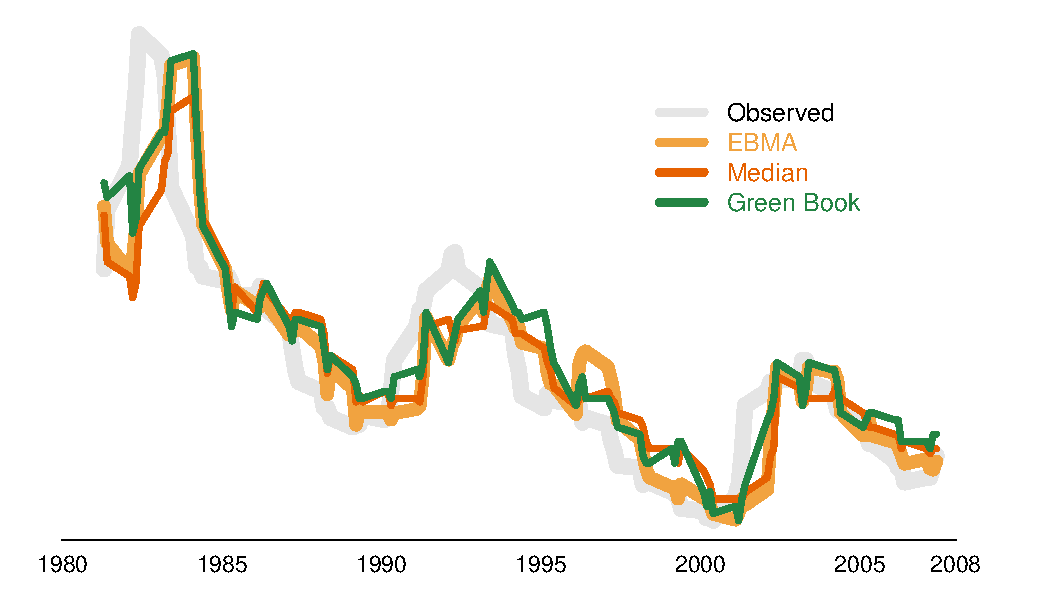
\includegraphics[scale=.65]{mdwtimeSeries2}
\end{center}

}


\frame{\frametitle{Predicting the Incumbent Voteshare in the 2012 Presidential Election -- Calibration Sample}     

\begin{center}
\begin{footnotesize}
\begin{tabular}{rlrrrrrrrrr}
\toprule
  & F & A & C & H & LBRT & L & Hol & EW & Cuz \\ 
\midrule
  1992 & 55.7 & 46.3 & 49.7 & 48.9 & 47.3 &  &  &  &  \\ 
  1996 & 49.5 & 57.0 & 55.5 & 53.5 & 53.3 &  & 57.2 & 55.6 &  \\ 
  2000 & 50.8 & 53.2 & 52.8 & 54.8 & 55.4 & 60.3 & 60.3 & 55.2 &  \\ 
  2004 & 57.5 & 53.7 & 52.8 & 53.2 & 49.9 & 57.6 & 55.8 & 52.9 & 51.1 \\ 
  2008 & 48.1 & 45.7 & 52.7 & 48.5 & 43.4 & 41.8 & 44.3 & 47.8 & 48.1 \\ 
\bottomrule
\end{tabular}
\end{footnotesize}
\end{center}


}


\frame{\frametitle{Model Weights and In-Sample Fit Statistics for EBMA Model of U.S. Presidential Elections (1992-2008)}
\begin{center}
\begin{footnotesize}
\begin{tabular}{lrrrr}
\toprule
 & \shortstack{EBMA\\ Weight}&RMSE &MAE \\ 
\midrule
EBMA &  & 1.92 & 1.56 \\ 
  Fair & 0.02 & 5.53 & 4.58 \\ 
  Abramowitz & 0.78 & 2.02 & 1.72 \\ 
  Campbell  & 0.07 & 3.46 & 2.88 \\ 
  Hibbs  & 0.04 & 2.68 & 2.44 \\ 
  Lewis-Beck, Rice, and Tien & 0.06 & 2.78 & 2.28 \\ 
  Lockerbie  & 0.00 & 7.33 & 6.97 \\ 
 Holbrook & 0.01 & 5.73 & 4.77 \\ 
  Erikson and Wlezien & 0.02 & 2.74 & 2.25 \\ 
  Cuz\`an & 0.00 & 1.27 & 0.95 \\ 
\bottomrule
\end{tabular}
\end{footnotesize}
\end{center}
}


\frame{
\begin{center}
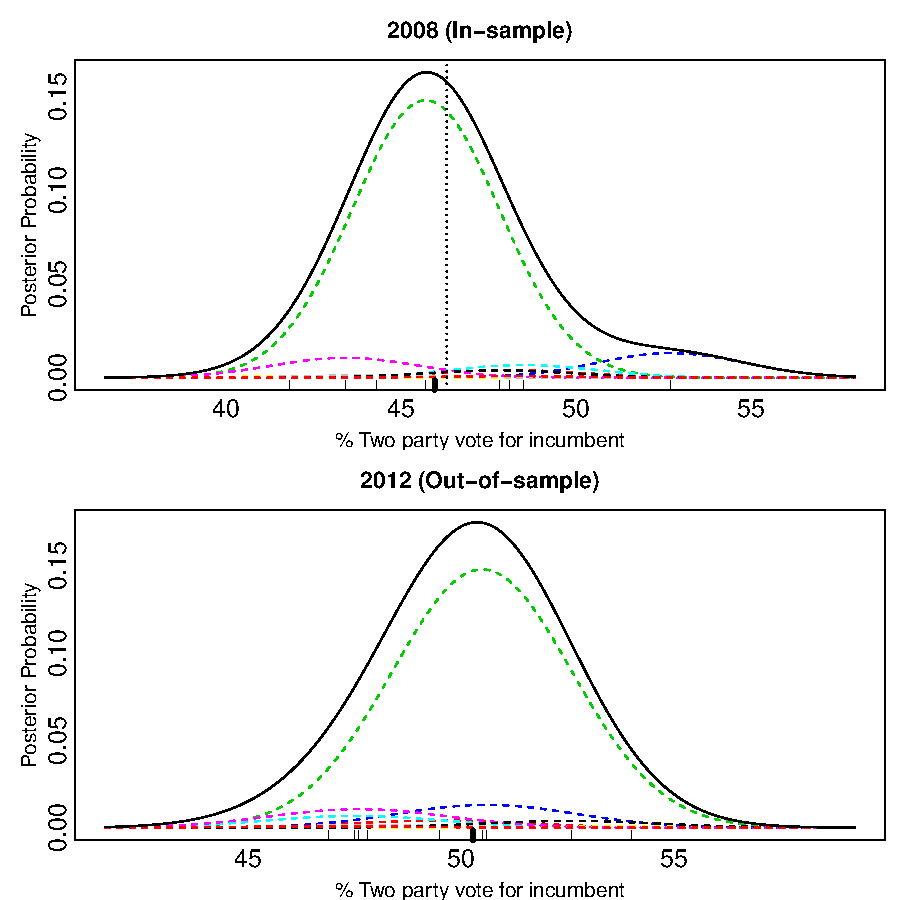
\includegraphics[scale=.6]{presForecast}
\end{center}

}


\frame{
\begin{center}
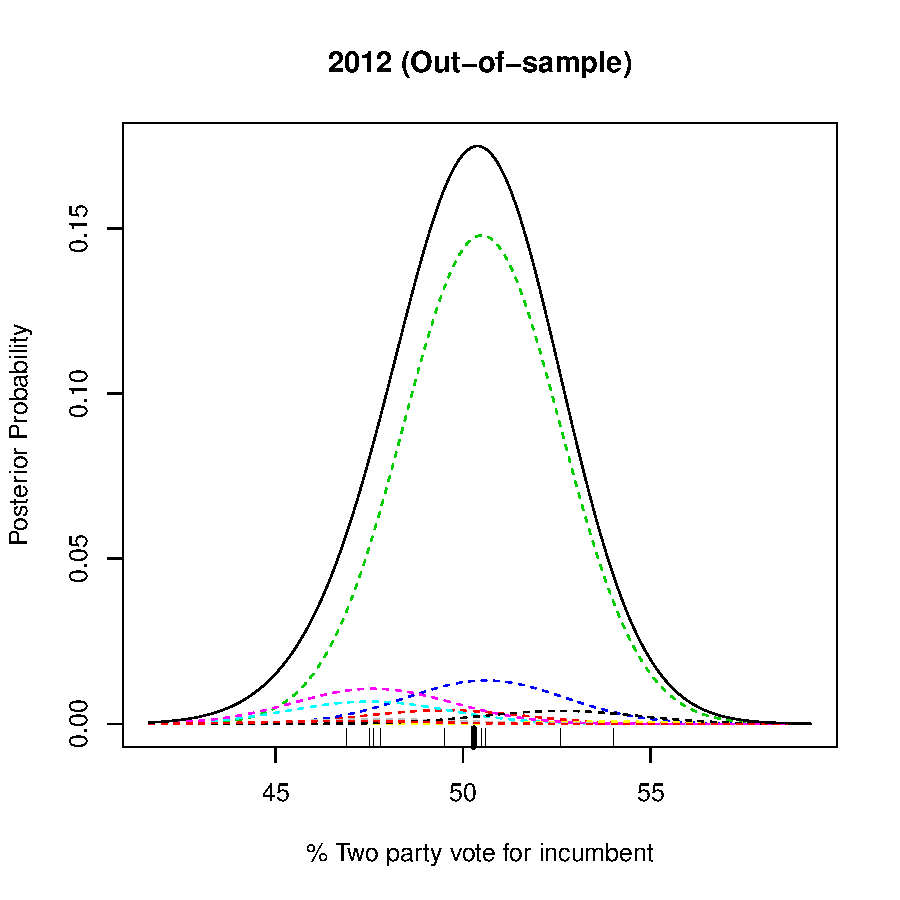
\includegraphics[scale=.6]{presForecast2012}
\end{center}

50.5, [46.52 - 54.2]


}



\end{document}\bye

